\chapter{Implementacja}
\label{cha:implementacja}
W ramach niniejszej pracy magisterskiej stworzono grę elektroniczną, w~której miał zostać wykorzystany przygotowywany prototyp interfejsu do  odczytu zmianów stanów emocjonalnych i~zachowań gracza. Na podstawie analizy silników do tworzenia gier przeprowadzonej w~rozdziale~\ref{cha:specyfikacja} zdecydowano się na wykorzystanie silnika Unity. Głównym powodem takiej decyzji była przede wszystkim ilość materiałów o~tematyce tworzenia gier przy pomocy właśnie silnika Unity, a~także dostępność rozwiązań, które pozwalały na prostą komunikację z~urządzeniami opisanymi w~rozdziale~\ref{cha:architektura}. 

\section{Podstawowe założenia}
Zanim rozpoczęto implementację gry, zostały określone założenia i~wymagania implementacyjne i~projektowe, według których następnie została zbudowana gra:
\begin{enumerate}
	\item Gra powinna zawierać mechaniki afektywne, które modyfikują rozgrywkę w~zależności od zachowania lub stanu emocjonalnego gracza.
	\item Jednym z~elementów implementacyjnych powinien być moduł umożliwiający komunikację z~urządzeniami opisanymi w~rozdziale~\ref{cha:architektura}. Moduł powinien także komunikować się z~serwerem zawierającym moduł do predykcji emocji oraz w~sposób prosty udostępniać zmiany stanu emocjonalnego użytkownika i~jego zachowań. 
	\item Gra powinna mieć możliwość wyboru jednego z~dwóch trybów gry: podstawowego, zawierający standardowe mechaniki gry, oraz wersję afektywną.
	\item Rozgrywka powinna być powtarzalna, tak aby w~trakcie przeprowadzania badań, każdy z~uczestników mógł doświadczyć tych samych elementów gry.
\end{enumerate}

\section{Implementacja gry}
%Opis gry, które elementy za co odpowiadają
Ponieważ przygotowywana gra miała być wykorzystana do przeprowadzenia eksperymentów w~celu ewaluacji opracowanego rozwiązania, zdecydowano, że będzie to gra jednoosobowa. W~trakcie rozgrywki gracz wciela się w~rolę kapitana statku kosmicznego, który musi walczyć z~przeciwnikami, aby przeżyć. Jego zadaniem jest sterowanie statkiem i~pokonanie jak największej liczby przeciwników przy pomocy dostępnego wyposażenia. Rozgrywka podzielona jest na poziomy, w~których trakcie gracz musi zdobyć określoną liczbę punktów. Na każdym z~poziomów dookoła statku generowanych jest kilka rodzajów wrogich statków, których schemat i~szybkość generowania są zróżnicowane w~zależności od poziomu. Z~każdym kolejnym poziomem pojawiają się nowe rodzaje jednostek, które mogą nie tylko wlatywać w~gracza lub do niego strzelać pojedynczymi pociskami, ale również wybuchać w~jego pobliżu, posiadać większą wytrzymałość lub strzelać innymi rodzajami pocisków. Każdy z~przeciwników ma także przypisaną ilość punktów, która jest dodawana do puli po zniszczeniu go. Aby przejść do kolejnego poziomu, gracz musi zebrać odpowiednią liczbę punktów.

Gracz posiada ograniczoną liczbę punktów życia, która zwiększa się po przejściu każdego z~poziomów. Aby urozmaicić rozgrywkę, dookoła gracza mogą pojawić się także wzmocnienia w~postaci innych broni oraz elementów leczących. Innym elementem mającym mocno wpłynąć na rozgrywkę jest moc specjalna, która umożliwia graczowi wypuszczenie fali w~kształcie okręgu, która natychmiastowo niszczy wrogie statki. Ponieważ umiejętność ta bardzo ułatwia rozgrywkę, gracz jest w~stanie użyć jej jedynie co określony czas. 

Aby wyrównać poziom gry i~nie znudzić gracz powtarzalną rozgrywką, każdy z~poziomów posiada także dodatkowy tryb, który jest trudniejszy niż podstawowa rozgrywka. Tryb ten jest uruchamiany na pewien określony czas po spełnieniu specjalnych warunków, które w~zależności od wersji gry są inne. W~trakcie trwania trybu trudnego schemat generowania przeciwników jest zmieniany na ich trudniejsze wersje, posiadające większą ilość życia i~inne umiejętności. Zmienia się także szybkość generowania przeciwników, która zostaje podwojona.

\begin{figure}
	\centering
	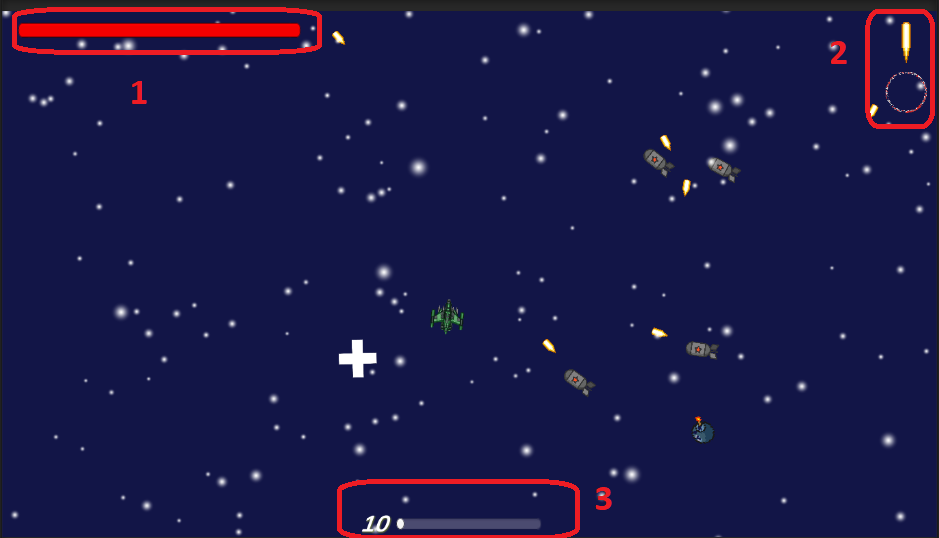
\includegraphics[width=0.7\linewidth]{images/ui.png}
	\caption{Ekran gry z~oznaczonymi elementami interfejsu użytkownika}
	\label{fig:ui}
\end{figure}

\section{Odczyt danych fizjologicznych i~zmian emocji}
Opis elementów do odczytu emocji i~EMG, odczyty z~cheststrapa, komunikacja z~serwerem

\section{Domknięcie pętli afektywnej}
Mechaniki, reakcja na konkretne emocje i~odczyty z~EMG, jak działa wersja bez emocji